\documentclass{article}
\usepackage{hyperref}
\usepackage{amsmath}
\usepackage{graphicx} % Required for inserting images
\usepackage{subcaption} %  for subfigures environments
\usepackage{float}
\usepackage[
 backend=biber,
 style=alphabetic,
 sorting=ynt
]{biblatex}
\addbibresource{references.bib}

\title{Photon Mapper}
\author{Javier Sancho Olano \\ \href{mailto:815520@unizar.es}{815520@unizar.es}}
\date{Junio 2024}

\begin{document}

\maketitle

\tableofcontents
\newpage

\section{Introducción}
La ecuación de render es una ecuación integral que describe la cantidad de
radiancia emitida de un punto \(\mathbf{x}\) de una superficie hacia una
dirección \(\mathbf{\omega_{o}}\)

\begin{equation}
L_o(\mathbf{x}, \mathbf{\omega_{o}}) = L_e(\mathbf{x}, \mathbf{\omega_{o}}) + \int_{\Omega} L_i(\mathbf{x}, \mathbf{\omega_{i}}) \cdot f_r(\mathbf{x}, \mathbf{\omega_{i}}, \mathbf{\omega_{o}}) \cdot  |\mathbf{n} \cdot \mathbf{\omega_{i}}| \, d\omega_{i}
\end{equation}

\begin{figure}[h]
    \centering
    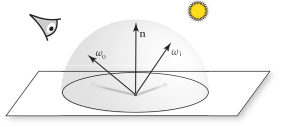
\includegraphics[width=0.6\textwidth]{imgs/rendereq.png}
    \caption{Ilustración del problema de la ecuación de render}
\end{figure}

En el reporte de \textit{path tracer} se explica cada termino de la ecuacion.

El algoritmo \textit{photon mapper} es un algoritmo de dos pasos que resuelve
esta ecuación. En el primer paso, se generan fotones que se trazan en la escena
desde las fuentes de luz. En el segundo paso, se trazan rayos desde la cámara y
al intersectar con la escena se calcula la radiancia en ese punto usando los
fotones generados en el paso anterior.

Con un número grande de fotones, tras el primer paso tendremos toda las escena
cubierta por fotones y por lo tanto, los fotones alrededor de un punto dado
darán una buena estimación de la radiancia incidente en ese punto.

La radiancia en un punto se define como\footnote{https://en.wikipedia.org/wiki/Radiance}:
\begin{equation} 
  L_i(\mathbf{x}, \mathbf{\omega_{i}}) = \frac{d^{2}\phi_{i}(\mathbf{x}, \mathbf{\omega_{i}})}{\cos\theta_{i} \: d\omega_{i} \: dA_{i}},
\end{equation}

dónde:
\begin{itemize}
  \item \(\mathbf{x}\) es un punto en el espacio
  \item \(\omega_{i}\) es la dirección de la radiancia incidente
  \item \(\phi_{i}(\mathbf{x}, \mathbf{\omega_{i}})\) es el flujo de los fotones en el punto \(\mathbf{x}\) en la dirección \(\mathbf{\omega_{i}}\)
  \item \(\cos\theta_{i}\) es el factor de corrección de la radiancia incidente
  \item \(A_{i}\) es el área de la superficie donde incide la radiancia
\end{itemize}

Con esto, podemos reescribir la ecuación de render como (omitiendo la radiancia
emitida):
\begin{equation}
\begin{split}
  L_o(\mathbf{x}, \mathbf{\omega_{o}}) & = \int_{\Omega} \frac{d^{2}\phi_{i}(\mathbf{x}, \mathbf{\omega_{i}})}{\cos\theta_{i} \: d\omega_{i} \: dA_{i}} \cdot f_r(\mathbf{x}, \mathbf{\omega_{i}}, \mathbf{\omega_{o}}) \cdot  |\mathbf{n} \cdot \mathbf{\omega_{i}}| \, d\omega_{i} \\
                                       & = \int_{\Omega} \frac{d^{2}\phi_{i}(\mathbf{x}, \mathbf{\omega_{i}})}{dA_{i}} \cdot f_r(\mathbf{x}, \mathbf{\omega_{i}}, \mathbf{\omega_{o}}) \\
\end{split}
\end{equation}

El flujo \(\phi_{i}\) se aproximará usando los \(n\) fotones más cercanos a
\(\mathbf{x}\) y cada fotón \(p\) tiene un flujo asociado \(\phi_{p}\).
\(\Delta A\) es el área de la superficie que cubre los \(n\) fotones, si \(r\)
es la distancia entre \(\mathbf{x}\) y el fotón más lejano, entonces
\(\Delta A = \pi r^{2}\). Entonces, aproximaremos la ecuación de render como:

\begin{equation}
\begin{split}
  L_o(\mathbf{x}, \mathbf{\omega_{o}})  & \approx \sum_{p=1}^{n} \frac{\phi_{p}}{\Delta A} \cdot f_r(\mathbf{x}, \mathbf{\omega_{p}}, \mathbf{\omega_{o}}) \\
                                        & \approx \frac{1}{\pi r^{2}} \sum_{p=1}^{n} \phi_{p} \cdot f_r(\mathbf{x}, \mathbf{\omega_{p}}, \mathbf{\omega_{o}})
\end{split}
\end{equation}

\section{Iluminación directa}
Vamos a comparar la iluminación directa con y sin \textit{next-event estimation}.
Para ello, usaremos la escena \textit{Cornell Box} con dos esferas de material
completamente difuso y una luz puntual. En la figura 2a, se muestra
la escena renderizada solo con el \textit{photon map} y en la figura
2b, se muestra la escena renderizada con el \textit{photon map} y
\textit{next-event estimation}.

\begin{figure}
\begin{subfigure}[h]{0.4\linewidth}
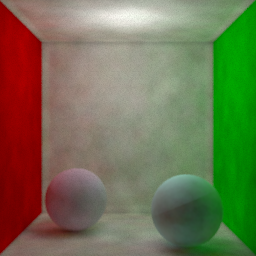
\includegraphics[width=\linewidth]{imgs/pml.png}
\caption{Iluminación directa sin next-event estimation}
\end{subfigure}
\hfill
\begin{subfigure}[h]{0.4\linewidth}
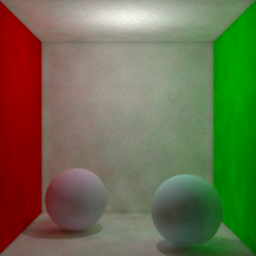
\includegraphics[width=\linewidth]{imgs/pmdl.png}
\caption{Iluminación directa con \textit{next-event estimation}}
\end{subfigure}
\caption{Cornell Box con 2 esferas difusas}
\end{figure}

La principal diferencia que observamos entre las dos imágenes son las
\textbf{\textit{hard shadows}}. El cálculo de la radiancia incidente con el \textit{photon map} genera una estimación sesgada. Esta situación se ilustra en la Figura 3, en un punto de transición, la radiancia incidente se estima con los fotones más cercanos, tanto en un lado de la sombra como en el otro. Esto suaviza la transición.

Por este motivo, el efecto de \textbf{\textit{soft shadows}} será muy fácil de obtener con el photon map.

\begin{figure}
\begin{subfigure}[h]{0.4\linewidth}
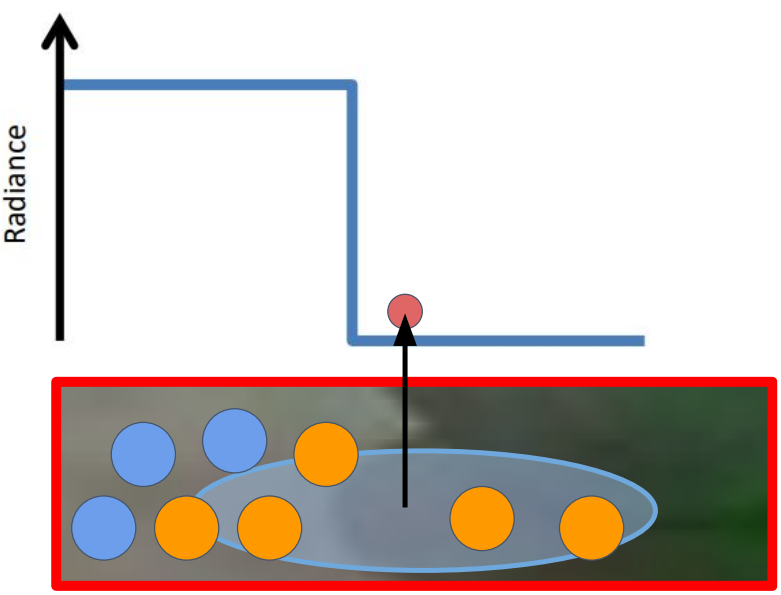
\includegraphics[width=\linewidth]{imgs/rad1.png}
\end{subfigure}
\hfill
\begin{subfigure}[h]{0.4\linewidth}
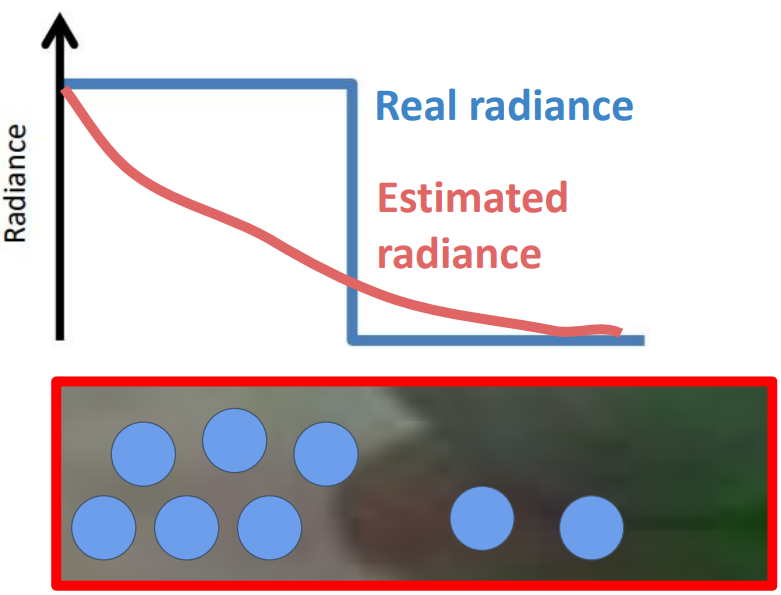
\includegraphics[width=\linewidth]{imgs/rad2.png}
\end{subfigure}
\caption{Ilustración de la estimacion sesgada de la radiancia incidente. Tomada de las diapositivas del laboratorio.}
\end{figure}

\section{Efectos de las BSDFs delta}
Para analizar los efectos de las BSDFs delta, vamos a renderizar la escena
\textit{Cornell Box} con una esfera de material plástico (difuso + especular),
otra esfera con un material de cristal (transmisiva y especular) y una luz
puntual.

\begin{figure}[H]
\centering
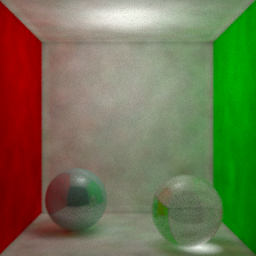
\includegraphics[width=0.6\linewidth]{imgs/pm_delta1.png}
\caption{Cornel Box con una esfera de cristal y otra de plastico}
\end{figure}

En primer lugar, una BSDF delta solo dispersara la radiación en una única dirección. Por lo que \(f_r(\mathbf{x}, \mathbf{\omega_{i}}, \mathbf{\omega_{o}})\) será siempre 0 para cualquier \(\mathbf{\omega_{i}}\) distinto de su único vector posible.

Sabiendo esto, el término \( f_r(\mathbf{x}, \mathbf{\omega_{p}}, \mathbf{\omega_{o}}) \) de la ecuación 4 será siempre 0 ya es muy improbable que un fotón de alrededor se encuentre en la dirección correcta. Por tanto, en la primera pasada del algoritmo, cuando un rayo se encuentre con una BSDF delta, seguirá el camino pero no guardará el fotón.

Por lo que todos los efectos de refracción y reflexión de la esfera de cristal
se computarán desde la parte de ray tracing, e.g: \textbf{\textit{cáusticas}}. 

Por otro lado, el efecto \textbf{\textit{color bleeding}} se consigue en la parte del photon mapping.

Además, el \textit{next-event estimator} se aplica en la parte del ray tracing por lo que las \textbf{\textit{hard-shadows}} se conseguirán en la parte de ray tracing.

\section{Resultados obtenidos}

Antes de empezar, vamos a analizar como el número de fotones y el número de vecinos afectan en el resultado analíticamente.
Dado un número de fotones \(N\), un "grado de infinitud" \(\alpha\) y las ecuaciones 3 y 4, podemos ver que:

\begin{equation}
\begin{split}
\lim_{N\to\infty} \sum_{p=1}^{\lfloor N^{\alpha}\rfloor} \frac{\phi_{p}}{\Delta A} \cdot f_r(\mathbf{x}, \mathbf{\omega_{p}}, \mathbf{\omega_{o}}) &= \int_{\Omega} \frac{d^{2}\phi_{i}(\mathbf{x}, \mathbf{\omega_{i}})}{dA_{i}} \cdot f_r(\mathbf{x}, \mathbf{\omega_{i}}, \mathbf{\omega_{o}}) \\
  &= L_o(\mathbf{x}, \mathbf{\omega_{o}})
\end{split}
\end{equation}

donde \(\lfloor N^{\alpha} \rfloor\) es el número de vecinos que se usaran para estimar la radiancia incidente. Este número nos permite justificar que el número de vecinos sera infinitamente mas pequeño que el número de fotones.
De esta forma obtenemos que la estimación de la radiancia sera precisa si el número de fotones tiende a infinito. \cite{HenrikCourse8}

En la practica esto no es posible, por lo que debemos tener un compromiso entre calidad de imagen y coste computacional. Vamos a ver como afectan estos parámetros en la calidad de la imagen:

\subsection{Número de fotones}
Dejando fijado el número de vecinos, aumentar el número de fotones provocara,
en primer lugar que los fotones estén mas repartidos por la escena y como resultado
que la estimación de la radiancia incidente sea mas precisa. Tal y como se puede ver en la ecuación 5, aumentar el número de fotones mejora la convergencia.

Naturalmente, el coste computacional aumentara ya que manejaremos muchos mas fotones.

\begin{figure}
\begin{subfigure}[h]{0.22\linewidth}
\includegraphics[width=\linewidth]{imgs/1k10kv.png}
\caption{N=1000. Patrón similar a una partición de Voronoi debido a la baja cantidad de fotones y un radio alto.}
\end{subfigure}
\hfill
\begin{subfigure}[h]{0.22\linewidth}
\includegraphics[width=\linewidth]{imgs/1k10k.png}
\caption{N=1000. Esta vez con un radio mas bajo se puede observar la distribución de los (pocos) fotones.}
\end{subfigure}
\hfill
\begin{subfigure}[h]{0.22\linewidth}
\includegraphics[width=\linewidth]{imgs/10k10k.png}
\caption{N=10,000.}
\end{subfigure}
\hfill
\begin{subfigure}[h]{0.22\linewidth}
\includegraphics[width=\linewidth]{imgs/100k10k.png}
\caption{N=100,000.}
\end{subfigure}

\caption{Cornell Box con k=10 y diferentes valores de N}
\end{figure}

\subsection{Número de vecinos}
Fijando el número de fotones, aumentar el número de vecinos provocara que la estimación de la radiancia incidente sea mas precisa, mejorando la convergencia. 

De igual forma, si el número de vecinos es muy grande, el coste computacional sera muy alto. 

\begin{figure}
\begin{subfigure}[h]{0.32\linewidth}
\includegraphics[width=\linewidth]{imgs/100k200k.png}
\caption{k=200.}
\end{subfigure}
\hfill
\begin{subfigure}[h]{0.32\linewidth}
\includegraphics[width=\linewidth]{imgs/100k1000k.png}
\caption{k=1,000.}
\end{subfigure}
\hfill
\begin{subfigure}[h]{0.32\linewidth}
\includegraphics[width=\linewidth]{imgs/100k2000k.png}
\caption{k=2,000.}
\end{subfigure}

\caption{Cornel Box con N=100,000 y diferentes valores de k}
\end{figure}

\section{Extensiones}
Además de todas la extensiones vistas en el reporte del \textit{path tracer}, he implementado:
\subsection{Kernels}

Si el radio de búsqueda es muy grande, la estimación de la radiancia puede ser imprecisa provocando que un aspecto borroso como se puede observar en la Figura 7a. Esto afectara de forma especialmente negativa a las cáusticas puesto que esperamos que estas tengan rayos de luz muy concentrados y nítidos.

Para reducir este efecto, usamos los kernels. Los kernels funcionan asignado un peso \(w_p\) a cada fotón en función de su distancia a \(\mathbf{x}\). Los kernels mas comunes son el kernel \textit{gaussiano} y el kernel \textit{conico}.

\begin{equation}
L_o(\mathbf{x}, \mathbf{\omega_{o}}) \approx \frac{1}{\pi r^2} \sum_{p=1}^{n} \phi_{p} \cdot f_r(\mathbf{x}, \mathbf{\omega_{p}}, \mathbf{\omega_{o}}) \cdot w_p
\end{equation}

\begin{figure}
\begin{subfigure}[h]{0.32\linewidth}
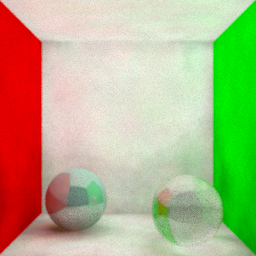
\includegraphics[width=\linewidth]{imgs/box.png}
\caption{Box kernel}
\end{subfigure}
\hfill
\begin{subfigure}[h]{0.32\linewidth}
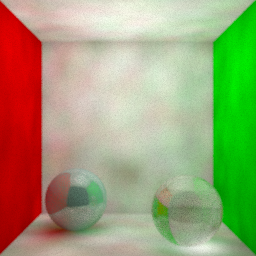
\includegraphics[width=\linewidth]{imgs/cone1.png}
\caption{Cone kernel}
\end{subfigure}
\hfill
\begin{subfigure}[h]{0.32\linewidth}
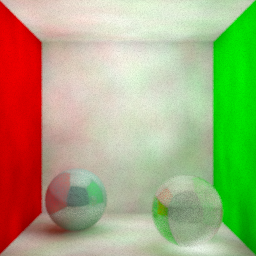
\includegraphics[width=\linewidth]{imgs/gaussian.png}
\caption{Gaussian kernel}
\end{subfigure}
\caption{Usar kernels para mejorar la estimacion de la radiancia}
\end{figure}

\subsubsection{Cone kernel}

\begin{equation}
w_p = \frac{1 - \frac{d_p}{k \cdot r}}{1 - \frac{2}{3k}},
\end{equation}

donde \(d_p\) es la distancia entre \(\mathbf{x}\) y el fotón \(p\), \(k \ge 1\) es una parámetro del kernel y \(r\) es la distancia máxima. \cite{HenrikCourse8}

El denominador de la ecuación 7 garantiza que el kernel este normalizado.

Por lo general un \(k\) bueno suele ser \(k=1\) y es el valor que he usado en la figura 7.

\subsubsection{Gaussian kernel}

\begin{equation}
w_p = \alpha \left[1 - \frac{1 - e^{-\beta\frac{d_p^2}{2r^2}}}{1 - e^{-\beta}} \right] ,
\end{equation}

Al igual que el \textit{cone kernel} este asignara mas peso a los fotones mas cercanos a \textbf{x} siguiendo la famosa curva gaussiana. A diferencia del  \textit{cone kernel} la pendiente sera mas suave y este efecto se puede ver en la figura 7.
He usado los parámetros \(\alpha = 0.918\) y \(\beta = 1.953 \) \cite{HenrikCourse8}
Este kernel ya esta normalizado por lo que la ecuación 6 seria:

\begin{equation}
L_o(\mathbf{x}, \mathbf{\omega_{o}}) \approx \sum_{p=1}^{n} \phi_{p} \cdot f_r(\mathbf{x}, \mathbf{\omega_{p}}, \mathbf{\omega_{o}}) \cdot w_p
\end{equation}


\medskip

\printbibliography

\end{document}
